\chapter{Results Discussion and Testing}
\section{General Overview}
To extract and classify entities, We used Stanford, NLTK and Polyglot. These entities extractor have common categories which are "Persons", "Location" and "Organization", Additionally NLTK and Stanford NER has another category which is called "others". This last category is not very clear. It combines numbers, percentage and unclassified entities. This can cause the confusion for to the organization. The core categories are those three first groups.

Among these three entities extractor, Stanford requires time to run compared to others.

The named entities must be set by the organization based on its interest. Some reports are composed by many pages but some few point must be highlighted. Templates in reporting are important, they made life easy.

Before extracting the entities, You must know what the document is  talking about. What the organization is struggling to know from the report.

Named entities from NLTK, Polyglot and Stanford are useful. They tried to summarise the primary information such as locations, persons and organizations. 

Sometimes, extracted named entities are not sufficient. Regular expressions can be used to respond perfectly the will of the organization.

\section{Case Study Results}
After analysing 1260 documents, Let us take one sample file and work on top section composed by 25 lines.

Consider a document which is specific to African region. "Africa regional office MDR60002 03 Nov2015.txt". We are requested to extract name of Persons who participated in IFRC activities.

We had a function to extract four categories of entities by Stanford NER. It is only to specify the category we are interested in. To identify persons names manually is also possible.
%\subsection{Stanford NER}
%\subsection{Polyglot}
%\subsection{Stanford}

\newpage
\section{Testing}\label{chp4}
For the security purpose testing gives a guarantee of correctness.  It is a major chapter for assertion of the research quality.

The process of extracting entities can be done in different ways. Either manually or by the use of machine learning algorithms. The manual way has many disadvantages as explained in Chapter \ref{Chapter2}.

Computer algorithms have impact for solving human problems. However we have to do a comparison for a small dataset between algorithm results and human results. The correctness of a tested dataset gives a confidence for remaining datasets.

IFRC uses the templates formats to produce their report. It is way of structuring a content of the document. The use of templates made most IFRC reports to have almost  the same size of top section. Top section contains important summary  as explained in Chapter \ref{top} .

Due to the time limitations, We tested  some  sample documents and We concluded for all top sections of the reports.
\section*{JSON file }
By taking the sample file, We extracted names of entities in JSON format. JSON stands for Java Script Object Notation. It is built based on two universal data structures such as a pair composed by a name and a value, and ordered list of values which is considered as an array, sequence, vector or list.
\begin{figure}[hbtp]
\caption{JSON File Structure \citep{bray2014javascript}}
\centering
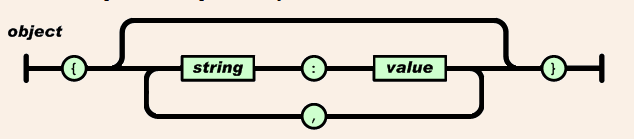
\includegraphics[scale=.7]{images/json.png}\label{json}
\end{figure}


Figure \ref{json}
refers to the structure of our json file. It contains a small dictionary which has one feature of proper names. We are able to identify three people who participate in IFRC sample report.
\newpage 
\begin{figure}[hbtp]
\centering
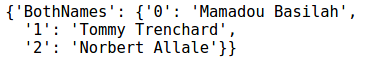
\includegraphics[scale=.7]{images/BothNames.png}
\caption{Persons Names Extracted by Hands}\label{Hand}
\end{figure}

After extracting three proper names as the Figure \ref{Hand} shows,  We are now going to do a comparison. We can compare the output of the algorithms.

\begin{figure}[hbtp]
\caption{Comparasion}
\centering
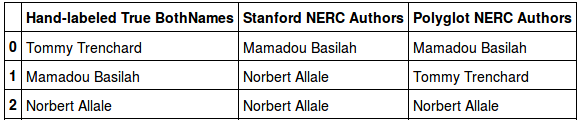
\includegraphics[scale=.8]{images/comparason.png}
\end{figure}


In Machine Learning, there are three ways of testing the quality of algorithms. As We extracted  entities from IFRC reports, to be sure on the work of algorithms,  We calculated recall, precision and accuracy. 

\textbf{Precision} has been calculated as a  fraction of relevant instances over  retrieved instances.

\textbf{Recall} has been gotten as a fraction of retrieved relevant instances over  sum of relevant instances.

%\textbf{Accuracy}

%\textbf{Accuracy}

Prediction is made by algorithms to predict the name of persons in sample document. The correctness can be calculated based on comparison between what predicted and what extracted by hands. The figure \ref{prediction} is  the results of comparison between Polyglot names of 
\begin{figure}[hbtp]
\caption{Precision}
\centering
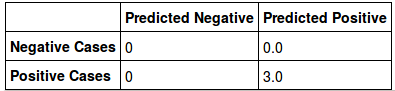
\includegraphics[scale=1]{images/precision.png}\label{prediction}
\end{figure}
